There exist two main approaches to modeling of the mechanical behavior of solid materials.
One approach is based on the continuum theory and the finite element method (FEM) is usually used for numerical solution, while the other approach considers the material as a set of discrete units (particles) and the discrete element method (DEM) is the main numerical solution method.
Both approaches have their fields of application, however, in certain cases they can be combined and used together.

The finite element method is a tool for approximate solution of partial differential equations.
In the context of solid mechanics, such equations describe the mechanical behavior of a \emph{continuous} material.
FEM underwent intensive development from both engineering and mathematical points of view and is being used for solution of various engineering and scientific problems.
Different enhancements and features (adaptive meshing, implicit/explicit solution schemes etc.) were investigated to reduce computational costs or improve usability and performance for different model features/purposes.
Despite these facts, FEM is considered not to be suitable for modeling of a large number of discontinuities (i.e., massive fragmentation), especially if a significant number of new contacts between individual \quotes{particles} is assumed.

The discrete element method (or particle models in other words) was originally developed for modeling of granular materials, i.e., \emph{discontinuous} matter.
Later on, the method was extended to bonded (or cohesive) particle models, resulting in a continuum-like behavior of discrete particles in the elastic range.
However, due to its discrete nature, beyond the elastic range the creation of discontinuities (like cracks, damage or even massive fragmentation) together with large displacement effects is very naturally included in the DEM formulation.
DEM is usually solved in an explicit sense, which allows easy computer implementation and straightforward contact law definitions, but makes the whole simulation computationally expensive at the same time.

The combination of FEM and DEM methods can be performed in several ways, depending on the context.
The vast majority of scientific papers dealing with this topic is aimed at concurrent FEM -- DEM coupling, i.e., modeling situations in which the process modeled by DEM and the process modeled by FEM take place at the same time and at least one of them influences the other.
Several classes of combination approaches have been developed, as will be discussed later.

In the concurrent approach (see chapter \ref{chapCouplingConcurent}), both DEM and FEM simulations have to run at the same time, increasing computational time costs.
In the case of multiscale coupling, each FEM integration point possesses its own DEM simulation (where the stress--strain law is determined from the actual microstructure evolution) and the computational costs grow even more due to this fact.

The classification complementary to the concurrent combination is the sequential approach.
It assumes that the processes are separable in time and therefore only the former process
(a bridge column subjected to an impact load, for example)
influences the latter process
(e.g., further bridge loading),
but not vice versa
(further bridge loading does not backward influence the impact).
In chapter \ref{chapCouplingSequential}, a DEM to FEM sequential mapping of damaged concrete material is presented.
Usually some kind of homogenization techique is used to determine FEM model parameters at the beginning of the latter
(e.g., further bridge loading)
process from the final state of the former
(e.g., an impact on the column)
process.

Concurrent coupling methods are computationally expensive.
On the other hand, the sequential mapping, due to its \quotes{one way} nature, allows, e.g., to use different FEM meshes while running the DEM part only once, reducing additional computation time.
Which approach is more suitable depends always on specific physical and simulation context.






\chapter{Concurrent DEM -- FEM coupling}\label{chapCouplingConcurent}

As an example of the concurrent coupling of the two methods, consider a dynamic soil compaction.
The compacted soil could be modeled by DEM, the compactor by FEM (here we have surface coupling) and the rest of the soil domain by FEM (soil is usually considered as continuous material on a larger scale).
The soil DEM / soil FEM interface would probably be of a volume coupling kind.
Of course, the FEM soil could be modeled using the multiscale approach, where a certain small representative volume around integration points of the FEM mesh is modeled by DEM (reflecting the discrete nature of the material on lower scale).
And we could go in coupling further and further\dots

This example was just to show the variety of possible coupling combinations and that there are a variety of real world problems, where such coupled methods could be useful.
Together with the simplicity of creating, modifying and running such simulations and extensibility of the used programs (due to the open source character of the code) it makes this approach attractive for a variety of engineering problems.

There are countless software programs for both FEM and DEM.
Some of them are commercial (usually) without possibility to change the code and adjust the behavior to our requirements (combination with another software for instance).
However, there exist programs with open source code, which the user can modify, possibly for coupling with other programs.
In the present work, coupling of FEM code \OOFEM\ \cite{PatzakBittnar2001a,oofemWWW} and DEM code \YADE\ \cite{Smilauer2010a,yade2010,yade2015,yadeWWW} is presented.
Both programs have the core written in C++ (providing efficient execution of time consuming routines), user interface written in Python (modern dynamic object oriented scripting language, providing easy to use scripting while preserving the C++ efficiency) and extensible object oriented architecture allowing independent implementation of new features - new material model or new particle shapes for instance.

Basic principles and examples of different coupling strategies (surface, volume, multiscale and contact coupling) are explained in the following sections.
All the methods and examples are considered as dynamic problems solved by an explicit scheme.
An implicit static solution would be possible, but with much more effort (DEM is not suitable for implicit schemes as discussed in the beginning of chapter \ref{chapDem}).
One example for each method is presented in this thesis. More examples should be available on the \github\ sites of the author.
The source code to the examples is available at \textfile{codes/external/fem-dem/examples} and on \github, too.






\section{Surface coupling}

\begin{figure}[htbp]
	\centering
	\includegraphics[width=8cm]{raphaelpy/coupling_illustration_surface}
	\begin{picture}(0,0)
		\setlength{\unitlength}{8cm}
		\put(-0.230769230769,0.0307692307692){\makebox(0,0){\small FEM}}
		\put(-0.830769230769,0.0307692307692){\makebox(0,0){\small DEM}}
		\put(-0.523076923077,0.446153846154){\makebox(0,0){\small load}}
		\put(-0.523076923077,0.2){\makebox(0,0){\small displacement}}
	\end{picture}
	\caption{Surface coupling illustration}
\end{figure}

The so called surface coupling
\cite{Munjiza2004a,OnateRojek2004a,VillardChevalierLeHelloCombe2009a,Fakhimi2009a,NakashimaOida2004a}
is probably the most straightforward FEM--DEM coupling strategy.

The principle is to split the whole problem into two separated domains, one modeled by FEM and the other by DEM.
As an illustrative example, consider a steel beam modeled by FEM falling into an assembly of gravel particles modeled by DEM.
Both domains interact with each other, but are physically separated during the entire time of the process.

If there exists a contact between a finite element and a DEM particle, the repulsive interaction force acts (with opposite direction) on both the DEM particle and on the FEM element.
The interaction forces are used as an external load for each domain.
The displacements of the FEM domain has to be taken into account in the DEM domain.

In the current \OOFEM/\YADE\ implementation, the boundary (surface) of the FEM mesh is copied into the DEM part as special triangular particles.
Then, in the case of explicit dynamic simulation, in each time step:
\begin{itemize}
	\item the DEM part is solved;
	\item the FEM part is solved;
	\item forces acting on DEM facets are interpolated into vertices and applied on FEM as nodal loads;
	\item positions of DEM facets are updated according to FEM displacements.
\end{itemize}


\subsection{Example}
This very simple example is aimed to test the approach, mainly correct contact detection and interaction evaluation.
A cantilever is \quotes{bombarded} by three particles.
One particle hits the cantilever \quotes{directly}, while two particles hit the cantilever outside its original position (one aspect of the testing).
The cantilever is modeled by FEM with linear brick elements. The bottom of the cantilever has fixed displacements.
The cantilever surface (set of quadrilateral faces) is triangulated and copied to the DEM part of the simulation.
The DEM \quotes{impactors} can have different shapes, e.g., spherical or polyhedral.
The visual results are shown in figure \ref{figCouplingConcurrentSurfaceExample1}, the animation can be found at \textfile{text/figs/couupling/surf1}.







\section{Volume coupling}

\begin{figure}[htbp]
	\centering
	\includegraphics[width=9cm]{raphaelpy/coupling_illustration_volume}
	\caption{Volume coupling illustration}
\end{figure}

Volume coupling \cite{RousseauFranginMarinDaudville2009a,XuGracieBelytschko2002a,AzevedoLemos2006a,WellmannWriggers2012a}
is similar to the surface coupling.
The difference is that the two subdomains overlap each other.

The possible usage of this approach could be a model of concrete beam subjected to an impact load (blast for example).
The whole beam would be modeled by FEM and only a small volume of the
concrete (the volume to be fragmented and crushed) would be modeled by DEM.
To preserve continuous nature of the beam, a transition zone (containing both FEM and DEM) would be included.

There are two basic strategies how to model transition between FEM and DEM domains \cite{XuGracieBelytschko2002a}.
The first one, \quotes{direct} or \quotes{master/slave} method \cite{AzevedoLemos2006a}, considers DEM particles overlapping with FEM as direct slaves of the FEM mesh (using standard \quotes{master/slave} or \quotes{hanging nodes} approach).
The second one, the \quotes{weak} or \quotes{Arlequin} method \cite{RousseauFranginMarinDaudville2009a,WellmannWriggers2012a}, considers a transition bridging zone, where the total response is superposed from contributions of the two models and is interpolated between both domains.
In the thesis, only the former (master/slave) approach is described.

In the current \OOFEM/\YADE\ implementation, hanging nodes are created at centers of overlapping spheres.
Then, in the case of explicit dynamic simulation, in each time step:
\begin{itemize}
	\item the DEM part is solved;
	\item the FEM part is solved;
	\item forces acting on DEM overlapping particles are applied on the corresponding FEM hanging nodes as nodal loads;
	\item position of overlapping DEM particles are updated according to displacements of the corresponding FEM hanging nodes.
\end{itemize}
% Jan Elias: wave propagation (!)

\subsection{Example}
In this example, a simply supported 2D beam subjected to a missile impact was simulated.
The sides of the beam body were simulated by FEM as a plane stress problem using quadrilateral elements and linear elastic material law.
The central part was modeled by DEM using a regular packing and CPM material model (described in section \ref{secDemCpm}).
The material parameters and initial conditions are artificially set to get \quotes{nice} results.
The visual results are shown in figure \ref{figCouplingConcurrentVolumeExample1}, the animation can be found at \textfile{text/figs/coupling/vol1}.




\section{Multiscale coupling}

\begin{figure}[hp]
	\centering
	\includegraphics[width=13cm]{raphaelpy/coupling_illustration_multiscale}
	\begin{picture}(0,0)
		\setlength{\unitlength}{13cm}
		\put(-0.85,0.1875){\makebox(-.03,0)[r]{IP}}
		\put(-0.6,0.34375){\makebox(0,0){strain}}
		\put(-0.6,0.03125){\makebox(0,0){stress}}
	\end{picture}
	\caption{Multiscale coupling illustration}
\end{figure}

The idea of multiscale simulations is to model the problem on the large (macro) scale using information from a lower (micro) scale \cite{RojekOnate2007a,WellmannWriggers2012a}.
In the current context, the (first order) homogenization \cite{GeersKouznetsovaBrekelmans2010a} is presented.

Geometric information (strain) from macro scale -- integration points (IPs) of FEM mesh -- is transferred to the micro scale (representative volume element - RVE - modeled by DEM).
On the micro scale, the boundary value problem (BVP) governed by the transferred prescribed strain is solved using periodic boundary conditions \cite{StranskyJirasek2011}.
The output of the micro-scale problem is the stress tensor (sufficient for explicit solution scheme) and possibly also the constitutive characteristics (stiffness tensor, needed by implicit solution schemes), which are transferred back to the macro-scale problem.

As an example of such approach, consider a sample of sand.
In reality, it is composed of individual grains, therefore DEM could be the right modeling approach.
However, because of very high computational costs of DEM, the sand is considered as a continuum from the macroscopic point of view and FEM is used for macroscopic description.
To preserve the particular nature of the sample, the stress--strain law in each integration point is determined not from predefined formulas,
but rather from microscale simulations performed on smaller sand samples solved by DEM.
Thus we do not need any explicit expression of the material law on the FEM scale (it is determined from the actual micro RVE response).

In the current \OOFEM/\YADE\ implementation, separate RVE is generated according to certain criteria for selected integration points.
Then, in the case of explicit dynamic simulation, in each time step:
\begin{itemize}
	\item the FEM part is solved;
	\item the DEM part is solved;
	\item strains at IPs are applied to the corresponding RVEs;
	\item stresses of RVEs are evaluated and adjusted to the corresponding IPs.
\end{itemize}



\subsection{Example}
Uniaxial strain (oedometric test) of a sample consisting of three different (linear elastic) materials is simulated in this example.
The macro-scale problem is modeled by three brick elements.
Each FEM element has eight integration points.
The upper one is a pure FEM element.
For each integration point of the two bottom elements, different DEM micro-scale RVE simulations are performed.

The visual results are shown in figure \ref{figCouplingConcurrentMultiExample1}, the animation can be found at \textfile{text/figs/coupling/multi1}.
In each \quotes{DEM} element, one micro RVE result is displayed.
The results of linear elastic behavior are not extremely spectacular indeed, but using a nonlinear behavior of RVEs (resulting in a higher stiffness when more inter-particle contacts occur for instance) could be very useful for certain applications.







\section{Contact coupling}

\begin{figure}[ht]
	\centering
	\includegraphics[width=10cm]{raphaelpy/coupling_illustration_contact}
	\begin{picture}(0,0)
		\setlength{\unitlength}{10cm}
		\put(-0.8,.03){\makebox(0,0){DEM}}
		\put(-0.2,.03){\makebox(0,0){FEM}}
	\end{picture}
	\caption{Contact coupling illustration}
\end{figure}

The idea of contact analysis \cite{Frenning2008a} is very simple and opposite to the multiscale approach.
The material on the large scale is considered to be of a particulate nature and is modeled by particles using DEM.
Each such particle is deformable and further modeled by FEM.

There is no strict border between the cases when the solution can be considered as a~contact FEM analysis and when it is already DEM.
For only a few particles we would probably use the former one, but when the number of particles increases, the DEM modeling (with its efficient contact detection algorithms) would be more appropriate.
This strategy can be actually considered as full FEM, only the contact detection and contact constitutive law is \quotes{borrowed} from the DEM program.

In the current \OOFEM/\YADE\ implementation, the FEM \quotes{particles} are copied into DEM part as polyhedrons.
Then, in the case of explicit dynamic simulation, in each time step:
\begin{itemize}
	\item the DEM part is solved;
	\item the FEM part is solved;
	\item forces acting on DEM polyhedrons are interpolated into vertices and applied on FEM as nodal loads;
	\item position and shape of DEM polyhedrons are updated according to the displacement of the FEM mesh.
\end{itemize}



\subsection{Example}

In this example, collision of three elastic bodies is presented.
All three particles are modeled by FEM, only a detection algorithm is borrowed from DEM.
The visual results are shown in figure \ref{figCouplingConcurrentContactExample1}, the animation can be found at \textfile{text/figs/coupling/contact1}.






\cleardoublepage
% to have color images on one sheet of paper, for printing

\begin{figure}[p]
	\centering
	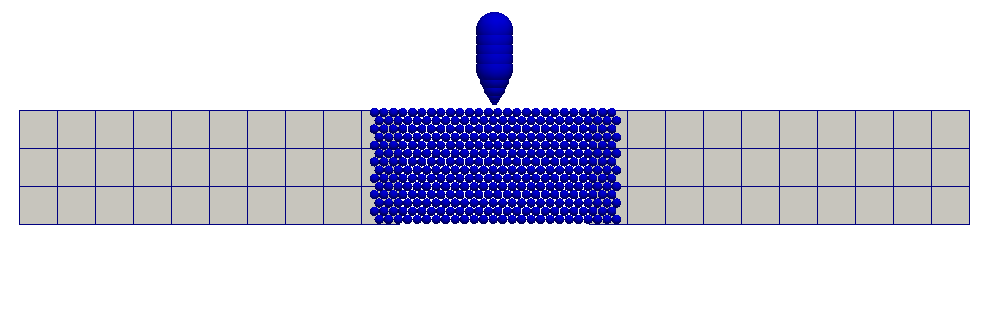
\includegraphics[width=15cm,trim={0 3.5cm 0 0cm},clip]{coupling/vol1/vol1-0000}
	\\
	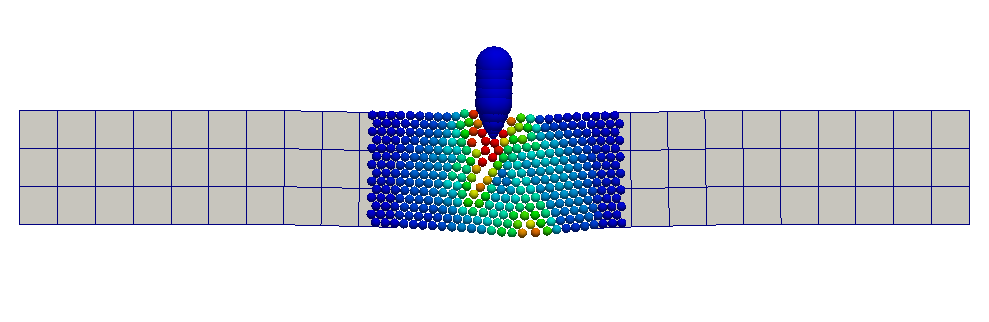
\includegraphics[width=15cm,trim={0 2.5cm 0 1.5cm},clip]{coupling/vol1/vol1-0020}
	\\
	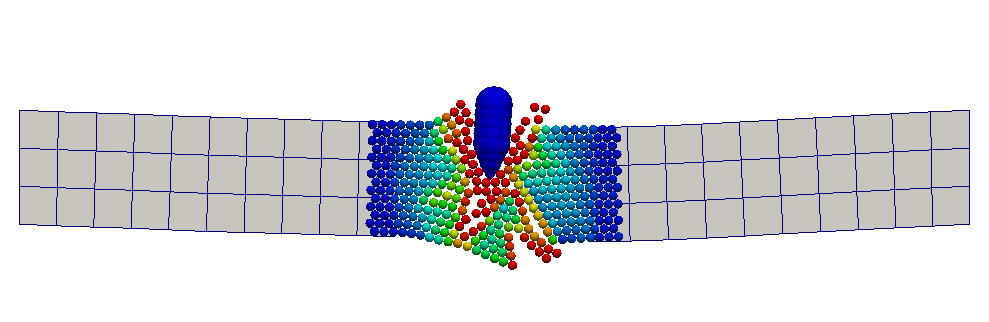
\includegraphics[width=15cm,trim={0 1.5cm 0 2.5cm},clip]{coupling/vol1/vol1-0050}
	\\
	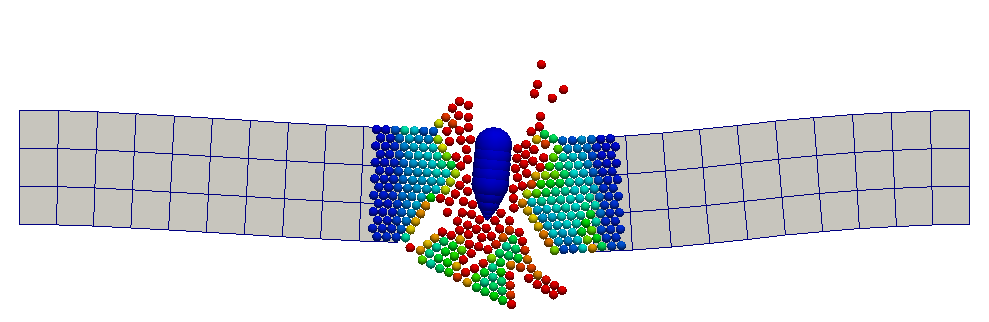
\includegraphics[width=15cm,trim={0 .0cm 0 2cm},clip]{coupling/vol1/vol1-0087}
	\caption{Impact on a simply supported beam at different stages}
	\label{figCouplingConcurrentVolumeExample1}
\end{figure}

\begin{figure}[p]
	\centering
	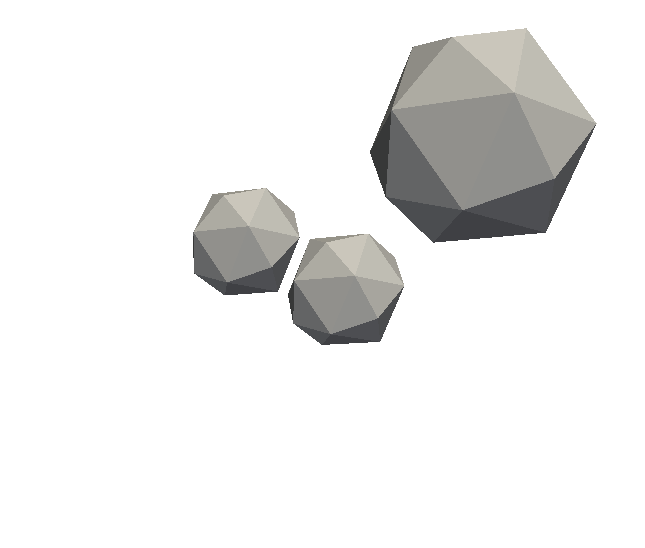
\includegraphics[width=5cm]{coupling/contact1/contact1-0010}
	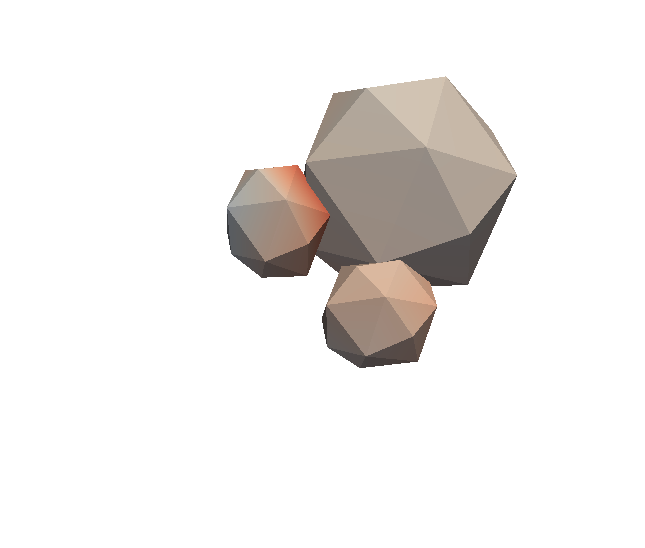
\includegraphics[width=5cm]{coupling/contact1/contact1-0053}
	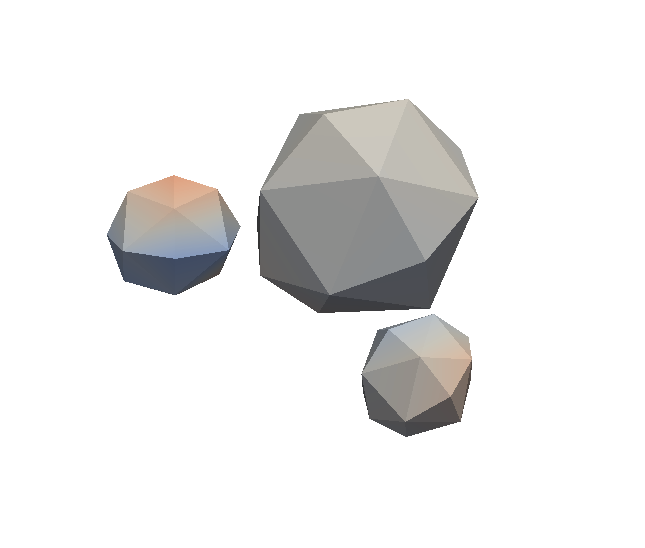
\includegraphics[width=5cm]{coupling/contact1/contact1-0080}
	\caption{Collision of three elastic particles at different stages}
	\label{figCouplingConcurrentContactExample1}
\end{figure}

\begin{figure}[p]
	\centering
	\includegraphics[width=5cm]{coupling/surf1/spheres/surf1-0000}
	\includegraphics[width=5cm]{coupling/surf1/spheres/surf1-0030}
	\includegraphics[width=5cm]{coupling/surf1/spheres/surf1-0060}
	\\
	\includegraphics[width=5cm]{coupling/surf1/poly/surf1-0000}
	\includegraphics[width=5cm]{coupling/surf1/poly/surf1-0030}
	\includegraphics[width=5cm]{coupling/surf1/poly/surf1-0060}
	\caption[Impact on a cantilever at different stages]{Impact on a cantilever at different stages. DEM particles can be spheres (top) or polyhedrons (bottom).}
	\label{figCouplingConcurrentSurfaceExample1}
\end{figure}

\begin{figure}[p]
	\centering
	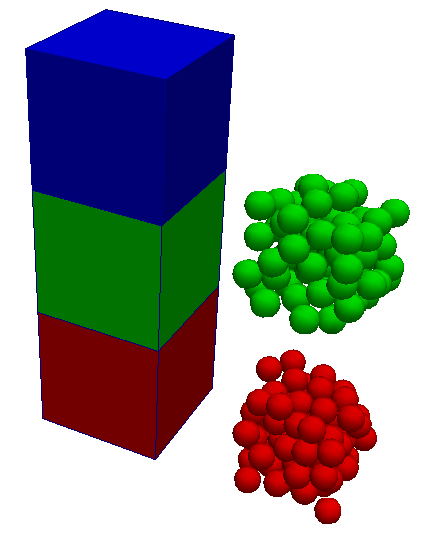
\includegraphics[width=5cm]{coupling/multi1/multi1-0000}
	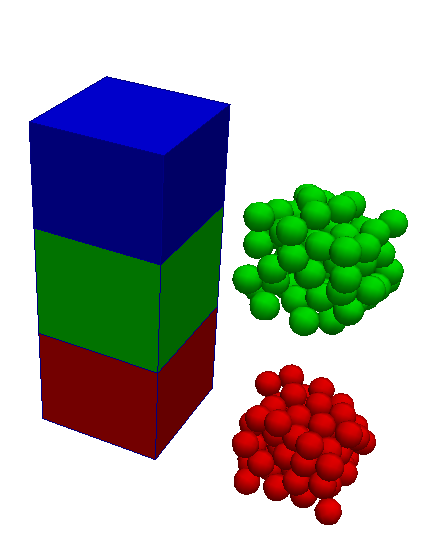
\includegraphics[width=5cm]{coupling/multi1/multi1-0025}
	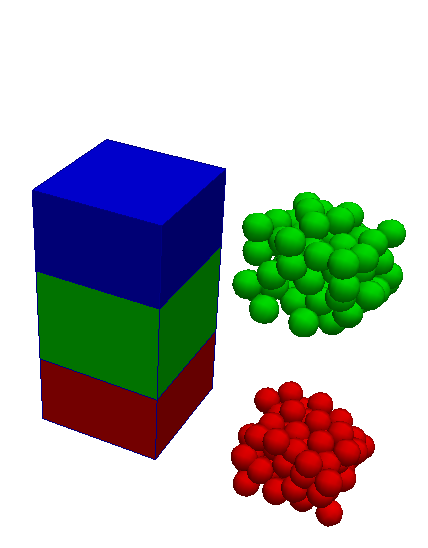
\includegraphics[width=5cm]{coupling/multi1/multi1-0050}
	\caption{Uniaxial strain test at different stages}
	\label{figCouplingConcurrentMultiExample1}
\end{figure}









%%%%%%%%%%%%%%%%%%%%%%%%%%%%%%%%%%%%%%%%%%%%%%%%%%%%%%%%%%%%%%%%%%%%%%
\chapter{Sequential DEM -- FEM coupling}\label{chapCouplingSequential}
In this chapter, a sequential mapping method from DEM to FEM applied to modeling of fracture of concrete is presented.
For example, consider
an impact load on a bridge column
and then
further bridge loading.
The two processes are clearly separable in time, where
the impact
influences
the behavior of the bridge under further loading,
but not vice versa.
From the physical nature,
the impact
is a dynamic process involving fragmentation and is therefore suitable for DEM.
On the other hand,
further bridge loading
could be a~(quasi)static \quotes{large-scale} process and is therefore suitable for FEM.
The aim of the mapping method is to take the information from a DEM simulation (e.g., damage and stress distribution) and use it within a FEM simulation.

The CPM, cohesive particle model for concrete \cite{Smilauer2010a}, is chosen for the DEM part.
CPM was developed for numerical modeling of concrete under dynamic loading with possibility of massive fragmentation (e.g., crushing) and can be used for simulations of
the impact influence.

The DPM, damage-plastic model for concrete failure \cite{GrasslJirasek2006a}, is chosen for the FEM part.
DPM was developed for numerical modeling of concrete under (quasi)static conditions and can be used for
further bridge loading
simulations.

Theoretically, both
impact
and
further bridge loading
processes could be modeled only with CPM model using DEM as a solution tool.
However, because of the aforementioned significant computational costs of DEM method, such approach is practically impossible and only a small volume around
the impact
directly subjected to fragmentation is modeled.
Similarly, FEM could be used for both
the impact
and
further bridge loading
simulations, but FEM was found, as already mentioned, not to be suitable for modeling of massive fragmentation, which is the case of
the impact.

As a conclusion, both methods are used to model different stages of concrete
bridge
lifetime.

According to the physical background of both CPM and DPM (see section \ref{secCouplingSequentialBackground}), the force/stress quantities and damage quantities have to be transferred from CPM to DPM.
The proposed method is based on microplane theory and homogenization of discrete forces into the continuous stress tensor and damage in discrete point into the continuous damage.
According to the knowledge of the author, no similar work is published in the literature.

The basics and features of both combined models are reviewed in section \ref{secCouplingSequentialBackground}.
The actual mapping method is described in section \ref{secCouplingSequentialTheory} and illustrated on simple examples in section \ref{secCouplingSequentialExamples}.




		
		
\section{Background}\label{secCouplingSequentialBackground}
In this section, the common features of as well as differences between the DPM and CPM models will be shown.
Based on the following equations and relations, the mapping process itself will be derived in section \ref{secCouplingSequentialTheory}.

\subsection{Damage--plastic model for concrete}
Some material models (e.g., the DPM model described below) consider the history of loading.
Commonly the concept of a model with internal variables is used.
Such internal variables (damage for instance) are evaluated and stored only at integration points.

The Damage-Plastic Model (DPM) for concrete \cite{GrasslJirasek2006a,ValentiniHofstetter2013a} is a continuum-based model for concrete failure combining the theories of plasticity and damage.
The model is described in detail in the aforementioned papers, thus only the basics of the model are summarized here.
This summary is mainly focused on the features used further for combination with the CPM model.

The combination of plasticity and isotropic damage is expressed in the constitutive stress-strain law
\begin{equation}
	\stressTensor = (1-\damage)\stressTensorEffective = (1-\damage)\tensor4{D}_e(\strainTensor-\strainTensorPlastic)
	,
	\label{eqDpmStressStrain}
\end{equation}
					where
$\stressTensor$ denotes stress,
$\stressTensorEffective$ effective stress,
$\damage$ damage,
$\tensor4{D}_e$ elastic stiffness,
$\strainTensor$ total strain,
$\strainTensorPlastic$ plastic strain
and $\strainTensor-\strainTensorPlastic = \strainTensorElastic$ elastic strain.


The plastic part of the constitutive law is governed by the yield function $f_p$ (which depends on all three invariants of the effective stress tensor $\stressTensorEffective$ and the hardening variable $\kappaP$) and a non-associated flow rule derived from the plastic potential $g_p$
\begin{align}
	f_p(\stressTensorEffective,\kappaP) &\le 0
	,
	&
	g_p(\stressTensorEffective,\kappaP) &\not= f_p(\stressTensorEffective,\kappaP)
	,
	&
	\dot{\kappaP} &= \dot{\kappaP}(\strainTensorPlasticRate)
	.
	\label{eqDpmPlasticity1}
\end{align}

\begin{figure}[ht]
	\centering
	\includegraphics[width=7cm]{raphaelpy/coupling_seq_cpm_dpm_2}
	\begin{picture}(0,0)
		\setlength{\unitlength}{7cm}
		\put(-0.1,0.1){\makebox(0,0)[l]{$\strain$}}
		\put(-0.9,0.566666666667){\makebox(0,0)[l]{$\stress$}}
		\put(-0.1,0.516666666667){\makebox(0,0)[l]{plasticity}}
		\put(-0.1,0.183333333333){\makebox(0,0)[l]{damage}}
		\put(-0.525,0.416666666667){\makebox(0,0)[l]{$\damage f_t$}}
		\put(-0.9,0.516666666667){\makebox(-.03,0)[r]{$f_t$}}
	\end{picture}
	\caption{Stress-strain diagram of DPM model in uniaxial tension.}
	\label{figDpmStressStrain}
\end{figure}

The damage part is expressed by the damage evolution function $g$ and the relationships between internal variables $\kappaD$ and $\kappaP$
\begin{equation}
	\text{damage}\left\{
	\begin{array}{cccl}
		\kappaP < 1 & \rr & \damage = 0 & (a) \\
		\kappaP = 1 & \rr & \damage = 0 & (b) \\
		\kappaP > 1 & \rr & \damage = g(\kappaD), \kappaD = \kappaP - 1 & (c).\\
	\end{array}
	\right.
	\label{eqDpmDamageEvolution}
\end{equation}
Damage evolution is driven by the plastic strain $\strainTensorPlastic$, see (\ref{eqDpmPlasticity1}) and (\ref{eqDpmDamageEvolution}).
If $\kappaP<1$ (\ref{eqDpmDamageEvolution}a), no damage occurs.
When $\kappaP=1$ (\ref{eqDpmDamageEvolution}b), the plasticity surface takes its final form.
After this point, $\kappaP>1$ (\ref{eqDpmDamageEvolution}c) and damage evolution begins.

The law is (due to damage and possible strain localization) dependent on the finite element size.

For the mapping part, the physical meaning of the damage variable $\damage$ is important.
As is expressed in equation (\ref{eqDpmStressStrain}) and visually in figure \ref{figDpmStressStrain}, the physical meaning of DPM damage is the relative reduction of effective stress (or in other words, the relative reduction of strength).


\subsection{Cohesive particle model for concrete}
The Cohesive Particle Model (CPM) for concrete (see \cite{Smilauer2010a} and section \ref{secDemCpm}) is a discrete model for concrete failure.
Figure \ref{figCpmStressStrain} recall the tensile response in normal direction.
The physical meaning of damage $\damage$ (unlike in the case of DPM model, see figure \ref{figCpmStressStrain}) is the stiffness reduction.
This difference between DPM and CPM is discussed more in detail in section \ref{subsecCouplingSequentialTheoryDamageConsistent}.

\begin{figure}[ht]
	\centering
	\includegraphics[width=7cm]{raphaelpy/coupling_seq_cpm_dpm_1}
	\begin{picture}(0,0)
		\setlength{\unitlength}{7cm}
		\put(-0.1,0.1){\makebox(0,0)[l]{$\strain$}}
		\put(-0.9,0.566666666667){\makebox(0,0)[l]{$\stress$}}
		\put(-0.714375,0.1715){\makebox(0,-.02)[t]{1}}
		\put(-0.6525,0.20725){\makebox(0,0)[l]{$(1-\damage)\linkMaterialStiffnessNormal$}}
		\put(-0.525,0.416666666667){\makebox(0,0)[l]{$\damageA f_t$}}
		\put(-0.733333333333,0.1){\makebox(0,-.02)[t]{$\strainO$}}
		\put(-0.525,0.1){\makebox(0,-.02)[t]{$\kappa$}}
		\put(-0.9,0.316666666667){\makebox(-.03,0)[r]{$r$}}
		\put(-0.9,0.516666666667){\makebox(-.03,0)[r]{$f_t$}}
	\end{picture}
	\caption{Uniaxial stress-strain diagram of one link of CPM model.}
	\label{figCpmStressStrain}
\end{figure}

% Jan Elias: what about shear?










\section{Theory}\label{secCouplingSequentialTheory}
In this section, the actual mapping method is described.
We want to transfer information from the CPM model
(used, e.g., for an impact simulation)
to the DPM model
(used, e.g., for further bridge loading simulations).
Because the starting model is discrete and the target model is continuum-based, the required operation is to map discrete quantities into their continuous counterparts.

\subsection{Stress tensor}
The stress tensor is computed according to equation \ref{eqDemDiscreteStressFinalStressExternalForces}. Because the considered FEM model is formulated for classical Boltzmann continuum, only the symmetric part is considered.
\begin{equation}
	\volume\stressTensor = \sym{\br{\sum_\externalp\positionVector\otimes\externalForceVector}}
	\label{eqCouplingSeqDiscreteStressTensor}
\end{equation}
$\volume$, $\externalp$, $\positionVector$ and $\externalForceVector$ denotes volume assigned to the particle, contact points, position vector of a~contact point and force acting on the particle at the contact point, respectively.



\subsection{Concrete damage}
For the purpose of damage mapping, we have to transform damage from both models into a variable with a consistent physical meaning.
Because the DPM model is the target of the mapping, the physical meaning of this model (the relative strength reduction) will be chosen.
Furthermore, the DPM model uses a scalar damage variable, whereas the CPM model represents damage of individual links containing also directional information.
We can therefore define the DEM damage in its tensorial nature.

\subsubsection{Consistent physical meaning}\label{subsecCouplingSequentialTheoryDamageConsistent}
The following derivation is based on figures \ref{figDpmStressStrain} and \ref{figCpmStressStrain}.
For each link, the CPM damage $\damage$ is converted to the DPM--like damage $\damageA$.
Firstly, the original and current tensile strengths ($f_{t}$ and $r$ respectively) are evaluated in terms of material properties $E$ and $\varepsilon_0$ and internal variables $\kappa$ and $\damage$:
\begin{align}
	f_{t} &= E\varepsilon_0,
	&
	r &= (1-\damage)E\kappa
	.
	\label{eqConsistentDamage1}
\end{align}
Comparing figures \ref{figDpmStressStrain} and \ref{figCpmStressStrain}, we can write
\begin{equation}
	\damageA = 1-\frac{r}{f_{t}} =
	1 - \frac{(1-\damage)E\kappa}{E\varepsilon_0} =
	1 - \frac{(1-\damage)\kappa}{\varepsilon_0}
	\label{eqConsistentDamageFinal}
\end{equation}
which is the expression of the CPM damage in the DPM physical meaning.



\subsubsection{Per-particle overall damage}
\begin{figure}[ht]
	\centering
	\includegraphics[width=9cm]{raphaelpy/coupling_seq_per_particle_damage}
	\begin{picture}(0,0)
		\setlength{\unitlength}{9cm}
		\put(-0.772980491288,0.581894147386){\makebox(0,.05)[t]{$\normalVector^\contact$}}
		\put(-0.67240873134,0.551722619402){\makebox(0,-.025)[rt]{$\damageA^\contact$}}
	\end{picture}
	\caption{Contact points, normals and damage.}
	\label{figDamage1}
\end{figure}

The derivation of the damage tensor is inspired by section \ref{secMacroPropertiesElasticAnalytical}.
We define the damage tensor $\damageTensor$ as a symmetric second-order tensor such that the difference between link damage $\damageA^\contact$ and the projection of the damage tensor $\damageTensor$ to the link direction $\normalVector^\contact$ is minimal in the least-square sense.
Note that the DPM--like damage quantity is used from now on.
In~mathematical terms, $\damageTensor$
minimizes the following function:
\begin{equation}
	\sum_\contact(\normalVector^\contact\cdot\damageTensor\cdot\normalVector^\contact - \damageA^\contact)^2 = \min
	,
	\label{eqDamageTensorMin}
\end{equation}
which means
\begin{equation}
	\begin{gathered}
		\bb{0} = \frac{\partial}{\partial \damageTensor}\left[\sum_\contact(\normalVector^\contact\cdot\damageTensor\cdot\normalVector^\contact - \damageA^\contact)^2\right] = \sum_\contact 2(\normalVector^\contact\cdot\damageTensor\cdot\normalVector^\contact - \damageA^\contact)\normalVector^\contact\otimes\normalVector^\contact =
		\\
		= 2\damageTensor : \sum_\contact\normalVector^\contact\otimes\normalVector^\contact\otimes\normalVector^\contact\otimes\normalVector^\contact - 2\sum_\contact\damageA^\contact\normalVector^\contact\otimes\normalVector^\contact
		\\
		\damageTensor : \sum_\contact\normalVector^\contact\otimes\normalVector^\contact\otimes\normalVector^\contact\otimes\normalVector^\contact = \sum_\contact\damageA^\contact\normalVector^\contact\otimes\normalVector^\contact
		.
	\end{gathered}
	\label{eqDamageTensorDiff}
\end{equation}

According to \cite{KuhlDAddettaLeukartRamm2001a} and equation (\ref{eqMacroPropertiesElasticTheorSumToIntegral}),
the approximation of a discrete set of normal vectors by uniformly distributed normals can be written as
\begin{equation}
	\frac{1}{N} \sum_\contact \normalVector^\contact\otimes\normalVector^\contact\otimes\normalVector^\contact\otimes\normalVector^\contact
	\approx
	\frac{1}{4\pi} \int_\Omega \normalVector^\contact\otimes\normalVector^\contact\otimes\normalVector^\contact\otimes\normalVector^\contact \idd{\Omega}
	\label{eqDiscreteToContNormal}
	.
\end{equation}
Substituting equation (\ref{eqDiscreteToContNormal}) into (\ref{eqDamageTensorDiff}) and using (\ref{eqAppendixMathUnitSphereIntegralNinjnknl}) (\ref{eqAppendixMathTensorsIdentity4symProperties}) and (\ref{eqAppendixMathTensorsVolProjDef}) we can write
\begin{equation}
	\begin{gathered}
		\damageTensor : (3\vol{\projectionTensor4} + 2\sym{\identityTensor4}) =
		\frac{15}{N} \sum_\contact\damageA^\contact\normalVector^\contact\otimes\normalVector^\contact
		\\
		3\vol{\damageTensor} + 2\damageTensor =
		\frac{15}{N} \sum_\contact\damageA^\contact\normalVector^\contact\otimes\normalVector^\contact
		.
	\end{gathered}
	\label{eqDamageTensorFinal}
\end{equation}

To solve equation (\ref{eqDamageTensorFinal}), firstly the trace of the damage tensor $\trace{\damageTensor}$ is evaluated with the help of identities (\ref{eqAppendixMathTensorsTraceOfVolumetricPartEqTraceOrig}) and (\ref{eqAppendixMathTensorsUnitVectorsTrNinj}):
\begin{equation}
	\begin{gathered}
		\trace{3\vol{\damageTensor} + 2\damageTensor} =
		\trace{\frac{15}{N} \sum_\contact\damageA^\contact\normalVector^\contact\otimes\normalVector^\contact}
		\\
		5\trace{\damageTensor} = \frac{15}{N}\sum_\contact\damageA^\contact
		\rr
		\trace{\damageTensor} = \frac{3}{N}\sum_\contact\damageA^\contact
		.
	\end{gathered}
	\label{eqCouplingSeqDiscreteDamageTensorTrace}
\end{equation}
This means that the mean value of the damage tensor
\begin{equation}
	\Omega_m = \frac{1}{3}\trace{\damageTensor} = \frac{1}{N}\sum_\contact\damageA^\contact
	\label{eqCouplingSeqDiscreteDamageTensorTraceEqMeanDmg}
\end{equation}
is the average of individual discrete damages, which has a clear physically meaning.

When the trace of the damage tensor $\trace{\damageTensor}$ is known according to (\ref{eqCouplingSeqDiscreteDamageTensorTrace}), the actual damage tensor can be expressed as:
\begin{equation}
	\begin{gathered}
		3\vol{\damageTensor} + 2\damageTensor =
		\trace{\damageTensor}\identityTensor2 + 2\damageTensor =
		\frac{15}{N} \sum_\contact\damageA^\contact\normalVector^\contact\otimes\normalVector^\contact
		\\
		\damageTensor = -\frac{1}{2}\trace{\damageTensor}\identityTensor2 + \frac{15}{2N}\sum_\contact\damageA^\contact\normalVector^\contact\otimes\normalVector^\contact
		= -\identityTensor2\frac{3}{2N}\sum_\contact\damageA^\contact + \frac{15}{2N}\sum_\contact\damageA^\contact\normalVector^\contact\otimes\normalVector^\contact
	.
	\end{gathered}
	\label{eqCouplingSeqDiscreteDamageTensor}
\end{equation}

As shown by equation (\ref{eqCouplingSeqDiscreteDamageTensorTraceEqMeanDmg}), the mean value of the damage tensor always equals the average damage, thus it is always in the range $[0,1]$.
However, its principal values may be negative or greater than 1, as shown in examples below.


\subsubsubsection{Examples}
The approach is illustrated on an artificial arrangement of axis aligned directions.
Table \ref{tabCouplinSeqPerPArticleDamageExample} shows computed principal values for different values of damage in different directions.
Because the presented damage tensor evaluation assumes uniform distribution of directions (which is not the case for 3 directions),
the results sometimes differ from intuitively expected values.
On the other hand, the examples naturally illustrates the possibility of negative values or values greater than 1.

Script \textfile{codes/scripts/damageTensor/example.py} shows convergence to expected results (the damage is artificially set as $\damageA^\contact=\normalVector^\contact\cdot\damageTensor\cdot\normalVector^\contact$) as the number of direction increases.

{
\newcommand{\myaxes}[3]{
	\includegraphics[width=2.5cm]{raphaelpy/myaxes}
	\begin{picture}(0,0)
		\setlength{\unitlength}{2.5cm}
		\put(-.8,.1){\makebox(0,0)[rb]{#1}}
		\put(-.2,.4){\makebox(0,0)[l]{#2}}
		\put(-.5,.7){\makebox(0,0)[l]{#3}}
	\end{picture}
}
\begin{table}
	\centering
	\caption{Principal values of damage tensor for various damages}
	\begin{tabular}{|C{3cm}|C{4cm}|C{2cm}|}
		\hline
		\myaxes{$\damage_x$}{$\damage_y$}{$\damage_z$} & ($\damageTensorI_x,\damageTensorI_y,\damageTensorI_z$) & $\displaystyle\frac{\trace{\damageTensor}}{3}$ \\
		\hline
		\hline
		\myaxes{0}{0}{0} & (0, 0, 0) & 0 \\
		\hline
		\myaxes{1}{1}{1} & (1, 1, 1) & 1 \\
		\hline
		\myaxes{0.5}{0.5}{0.5} & (0.5, 0.5, 0.5) & 0.5 \\
		\hline
		\myaxes{1}{1}{0} & (1.5, 1.5, -1) & $\dfrac{2}{3}$ \\
		\hline
		\myaxes{0.5}{0.5}{0} & (0.75, 0.75, -0.5) & $\dfrac{1}{3}$ \\
		\hline
		\myaxes{1}{0}{0} & (2, -0.5, -0.5) & $\dfrac{1}{3}$ \\
		\hline
		\myaxes{0.5}{0}{0} & (1, -0.25, -0.25) & $\dfrac{1}{6}$ \\
		\hline
	\end{tabular}
	\label{tabCouplinSeqPerPArticleDamageExample}
\end{table}
}





\subsection{Mapping}
Auxiliary formulas derived in the previous sections will be used in this section for the actual mapping.
The mapping method is sequential, i.e., firstly the DEM simulation is run and the stress tensor and damage tensor are saved for all particles.
This information is then included in the FEM simulation.
Both simulations can be run independently, e.g., the FEM simulation can be done with different meshes without the need of recomputing the DEM part, or the DEM part can be run independently of the FEM mesh.
This approach also allows to use independent averaging methods.

In DEM simulations, the stress tensor $\stressTensor$ and damage tensor $\damageTensor$ are computed for each particle according to formulas (\ref{eqCouplingSeqDiscreteStressTensor}) and (\ref{eqCouplingSeqDiscreteDamageTensor}), respectively.
Before the FEM simulation, the mesh to be used must be known (in particular the coordinates of integration points).
For each integration point, the stress tensor and damage tensor are averaged and passed to the FEM simulation.
The averaging may be of any type.

In the DPM part of the mapping, the following process is performed for each integration point.
The damage scalar is evaluated from the averaged damage tensor (in particular from its principal values), generally
\begin{equation}
	\damage = \damage(\damageTensor) = \damage(\damageTensorI_1,\damageTensorI_2,\damageTensorI_3)
	.
\end{equation}
The specific form of the $\damage(\damageTensorI_1,\damageTensorI_2,\damageTensorI_3)$ function is dependent on material properties and typical loading scenarios for given situation.

For the known damage scalar $\damage$, the corresponding internal variables $\kappaD$ and $\kappaP$ have to be evaluated.
Because the DPM damage law $\damage=g(\kappaD)$ (relating $\kappaD$ and $\damage$) is element-size dependent, the following operations are done, when the element size is already known:
\begin{equation}
	\left\{
		\begin{array}{cclll}
			\damage \le m & \rr & \kappaD = 0, & \kappaP = \kappaP(\damage), & \damage = 0 \\
			\damage > m & \rr & \kappaD = g^{-1}(\damage) & \kappaP = \kappaD + 1.
		\end{array}
	\right.
	\label{eqCouplingSeqKappaPBackdoor}
\end{equation}
For very low values of resulting damage, less than a certain $m$, the corresponding DPM material state would be plastic (before the onset of damage).
Therefore the first $\kappaP=\kappaP(\damage)$ is computed and then $\damage=0$ is further considered.
See the example in the next section for illustration.

At the beginning of the FEM simulation, the actual total strain is not known.
Therefore we assume the total strain to be zero.
To preserve the elastic strain consistent with the stress tensor, a fictitious value of the plastic strain tensor (i.e., a value which does not necessarily correspond to the real physical plastic strain) is evaluated according to the DPM stress--strain law (\ref{eqDpmStressStrain}):
\begin{equation}
	\stressTensor = (1-\damage)\tensor4{D}_e:(\strainTensor-\strainTensorPlastic)
	\overset{\strainTensor=\tensor2{0}}{\rr}
	\strainTensorPlastic = -\frac{1}{1-\damage}\tensor4{D}_e^{-1}:\stressTensor
\end{equation}
The evaluated plastic strain therefore corresponds to the real plastic strain minus the unknown initial total strain.

After this point, the FEM simulation is run in the usual way.


\section{Example - uniaxial compression}\label{secCouplingSequentialExamples}
In this section, the results of proposed method are shown on simple \quotes{one element} tests.
The simulated prismatic specimen is subjected to uniaxial compression.
In the case of a one-element FEM simulation, the definition of boundary conditions is straightforward.
In~the DEM simulation, the axial strain is imposed by prescribed displacements at the top and bottom boundary layers.
In the lateral directions, the particles are free to move.
For the graphical post-processing, the stress values from DEM simulation are obtained as the normal component in the axial direction of the average stress.

The DEM and FEM material parameters are set such that the resulting stress-strain diagrams are as similar as possible.
Figure \ref{figCouplingSequantialResultsPlain} shows a very good agreement of the two models in both pre-peak and post-peak regime.
However, the two models differ at the peak load (the CPM softening starts prior to the DPM softening).

The DEM specimen is loaded at a certain level and then possibly unloaded.
At the final stage of the DEM simulation, relevant quantities are mapped onto the one-element FEM simulation and the FEM simulation is run.
The average stress tensor and average damage tensor are evaluated from all \quotes{ordinary} particles (not belonging to the layer imposing boundary conditions).

Based on numerical testing, the damage transformation law
\begin{equation}
	\damage = 2{.}09\br{0{.}85\damageTensorI_1+0{.}15\damageTensorI_3}^{4{.}7}
	\label{eqCouplingSeqDmgTransformation}
\end{equation}
was chosen.
$\damageTensorI_1$ denotes the maximum principal value of the damage tensor and $\damageTensorI_3$ the minimum one.
See figure \ref{figCouplingSequantialResultsDmg}.

For the DPM plastic stage before damage onset (\ref{eqCouplingSeqKappaPBackdoor}),
\begin{equation}
	\text{if}\quad \damage \le m \quad \text{then}\quad \kappaD = 0, \kappaP = \kappaP(\damage), \damage = 0
	,
\end{equation}
the following value and formula
\begin{align}
	m &= 5\cdot10^{-4}
	&
	\kappaP &= 0{.}3 + 900\damage
\end{align}
were chosen after numerical testing.

Graphs in figures \ref{figCouplingSequantialResultsMappingMonotonic} and \ref{figCouplingSequantialResultsMappingUnloaded} show results of the CPM simulation (grey) and continuation with the mapped DPM model (black).
The presented results show a reasonable approximation of the FEM behavior after the transformation from DEM.
The biggest error is obtained, if the mapping occurs around the peak (or after unloading from around the peak) where the results of two presented models differ the most.

\begin{figure}
	\centering
	\inputplot{sequential_coupling_plain}
	\caption{Stress-strain diagrams for individual models}
	\label{figCouplingSequantialResultsPlain}
\end{figure}

\begin{figure}
	\centering
	\inputplot{sequential_coupling_dmg}
	\caption{Chosen damage transformation law reflecting residual strength of CPM model}
	\label{figCouplingSequantialResultsDmg}
\end{figure}

\begin{figure}
	\centering
	\inputplot{sequential_coupling_001}
	\inputplot{sequential_coupling_002}
	\inputplot{sequential_coupling_003}
	\inputplot{sequential_coupling_004}
	\inputplot{sequential_coupling_005}
	\inputplot{sequential_coupling_006}
	\caption{Results of mapping at monotonic loading}
	\label{figCouplingSequantialResultsMappingMonotonic}
\end{figure}

\begin{figure}
	\centering
	\inputplot{sequential_coupling_007}
	\inputplot{sequential_coupling_008}
	\inputplot{sequential_coupling_009}
	\inputplot{sequential_coupling_010}
	\inputplot{sequential_coupling_011}
	\caption{Results of mapping at unloaded state}
	\label{figCouplingSequantialResultsMappingUnloaded}
\end{figure}

% Jan Elias: only uniaxial compression is promising, but expected more results here
